\documentclass{article}

\usepackage{graphicx}
\usepackage{tikz}
\usepackage{tikzsymbols}
\usetikzlibrary{calc,patterns,shapes.geometric}
\pagestyle{empty}
\usepackage[margin=0pt]{geometry}
\geometry{papersize={14in,12in}}

\def\centerarc[#1](#2)(#3:#4:#5){\draw[#1] ($(#2)+({#5*cos(#3)},{#5*sin(#3)})$) arc (#3:#4:#5);}

\begin{document}
	\begin{figure}
		\centering
		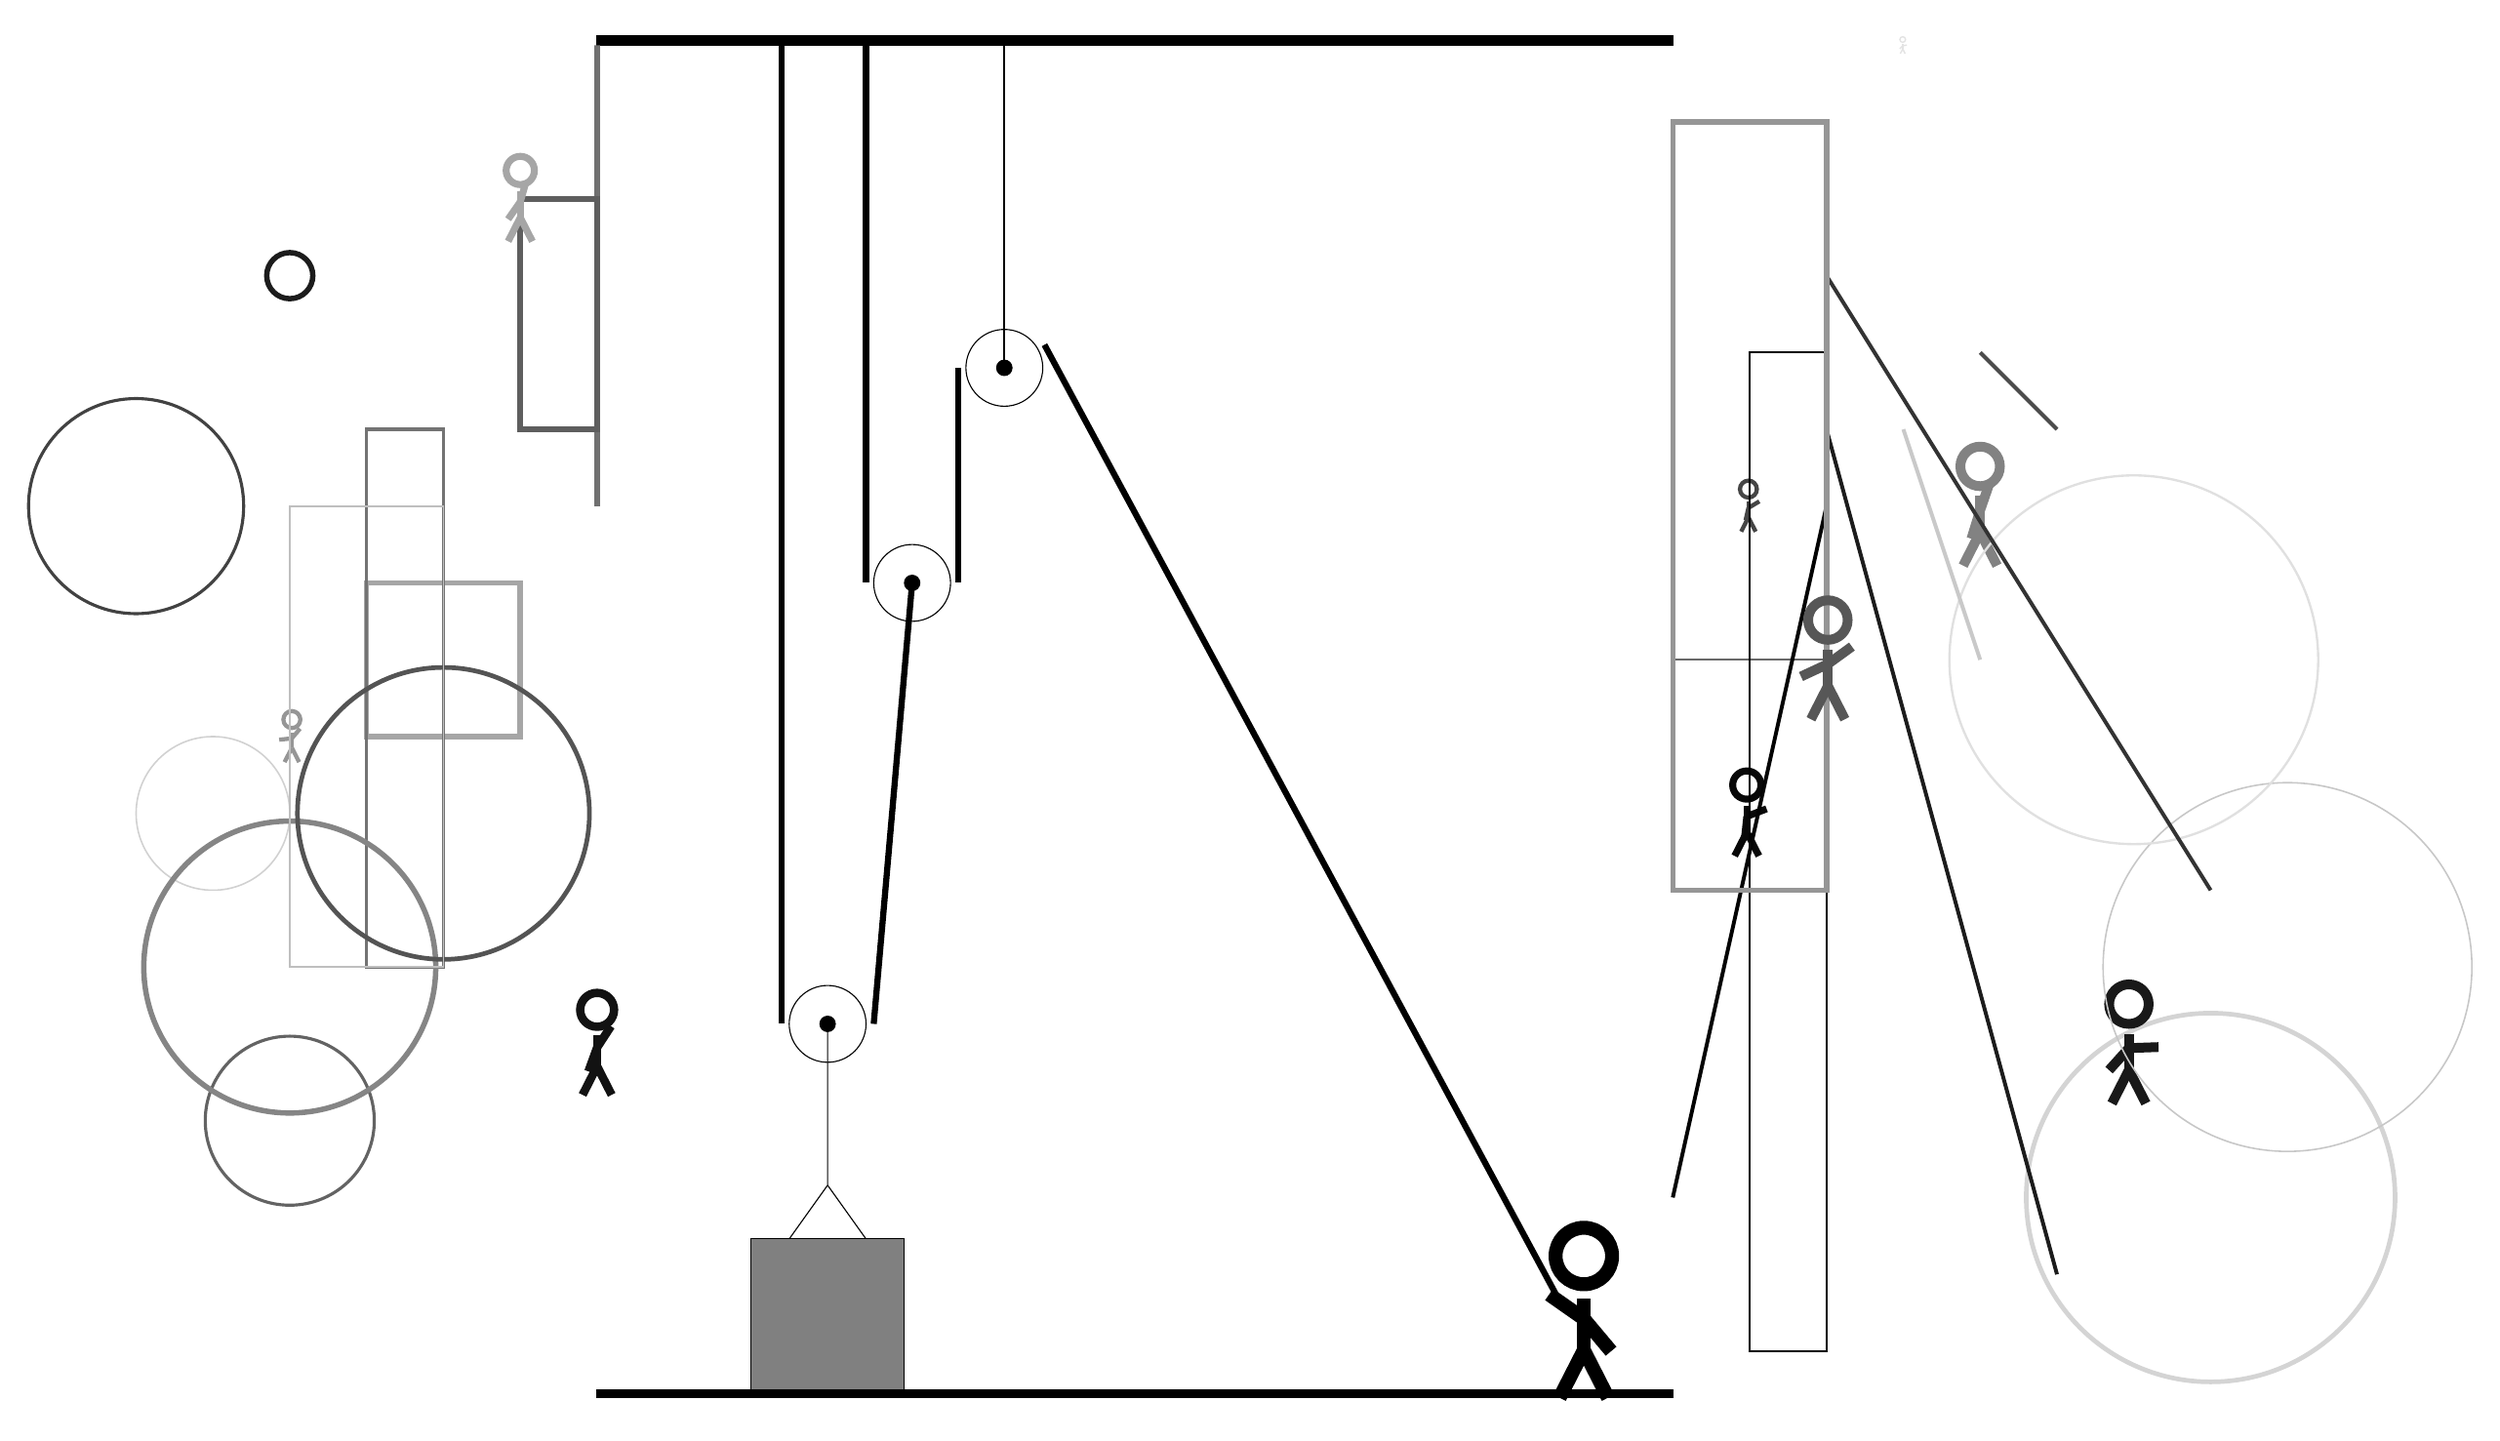
\begin{tikzpicture}
			%%%%% START %%%%%
			
			\draw[fill=black] (-2, 14) rectangle (12, 14.125);
			
			\draw (1, 1.26) circle (0.5);
			\draw[fill=black] (1, 1.26) circle (0.1);
			
			\draw (2.1, 7.0) circle (0.5);
			\draw[fill=black] (2.1, 7.0) circle (0.1);
			
			\draw (3.3, 9.8) circle (0.5);
			\draw[fill=black] (3.3, 9.8) circle (0.1);
			\draw[thick] (3.3, 9.8) -- (3.3, 14);
			
			\draw (1, 1.26) -- (1, -0.84) -- (0.5, -1.54) -- (1.5, -1.54) -- (1, -0.84);
			\draw[fill=black!50] (0, -1.54) rectangle (2, -3.54);
			
			\draw[line width=0.8mm] (0.4, 14) -- (0.4, 1.26);
			\centerarc[line width=0.8mm](1, 1.26)(180:360:0.6);
			\draw[line width=0.8mm](1.6, 1.26) -- (2.1, 7.0);
			\draw[line width=0.8mm] (1.5, 14) -- (1.5, 7.0);
			\centerarc[line width=0.8mm](2.1, 7.0)(180:360:0.6);
			\draw[line width=0.8mm](2.7, 7.0) -- (2.7, 9.8);
			\centerarc[line width=0.8mm](3.3, 9.8)(30:180:0.6);
			\draw[line width=0.8mm] (3.822, 10.1) -- (10.5, -2.3);
			
			\node at (10.8, -2.5) {\Strichmaxerl[10][-35][-50]};
			
			\node[line width=0.4mm, color=black!41] at (-6, 5) {\Strichmaxerl[3][6][50]};
			
			\draw[line width=0.7mm, color=black!56] (-2, 14) rectangle (-2, 8);
			\draw[line width=0.7mm, color=black!35] (-3, 7) rectangle (-5, 5);
			\draw [line width=0.6mm, color=black!17](19, -1) circle (2.4);
			\node[line width=0.3mm, color=black!90] at (18, 1) {\Strichmaxerl[7][48][2]};
			\node[line width=0.7mm, color=black!11] at (15, 14) {\Strichmaxerl[1][45][10]};
			
			\node[line width=0.5mm, color=black!73] at (13, 8) {\Strichmaxerl[3][77][31]};
			\draw[line width=0.4mm, color=black!55] (-4, 2) rectangle (-5, 9);
			\draw [line width=0.4mm, color=black!61](-6, 0) circle (1.1);
			\draw [line width=0.2mm, color=black!18](-7, 4) circle (1.0);
			
			\draw [line width=0.4mm, color=black!74](-8, 8) circle (1.4);
			
			\draw [line width=0.7mm, color=black!48](-6, 2) circle (1.9);
			\node[line width=0.4mm, color=black!49] at (16, 8) {\Strichmaxerl[7][73][71]};
			
			\draw [line width=0.6mm, color=black!67](-4, 4) circle (1.9);
			\draw [line width=0.2mm, color=black!22](20, 2) circle (2.4);
			\draw [line width=0.3mm, color=black!12](18, 6) circle (2.4);
			\draw[line width=0.5mm, color=black!89](14, 9) -- (17, -2);
			\node[line width=0.3mm, color=black!93] at (-2, 1) {\Strichmaxerl[6][70][57]};
			\node[line width=0.7mm, color=black!97] at (13, 4) {\Strichmaxerl[5][84][21]};
			\draw[line width=0.2mm, color=black!59] (14, 13) rectangle (12, 6);
			\draw[line width=0.2mm, color=black!25] (-4, 2) rectangle (-6, 8);
			
			\draw[line width=0.5mm, color=black!80](14, 11) -- (19, 3);
			\draw[line width=0.7mm, color=black!63] (-2, 9) rectangle (-3, 12);
			\draw[line width=0.2mm, color=black!99] (14, -3) rectangle (13, 10);
			\draw[line width=0.5mm, color=black!21](16, 6) -- (15, 9);
			
			\draw[line width=0.5mm, color=black!99](14, 8) -- (12, -1);
			\draw [line width=0.7mm, color=black!89](-6, 11) circle (0.3);
			\node[line width=0.7mm, color=black!35] at (-3, 12) {\Strichmaxerl[5][55][74]};
			
			\draw[line width=0.7mm, color=black!41] (12, 13) rectangle (14, 3);
			\node[line width=0.2mm, color=black!66] at (14, 6) {\Strichmaxerl[7][25][36]};
			\draw[line width=0.5mm, color=black!70](16, 10) -- (17, 9);
			
			
			\draw[fill=black] (-2, -3.5) rectangle (12, -3.6);
			
			%%%%% END %%%%%
		\end{tikzpicture}
	\end{figure}	
\end{document}